\documentclass[12pt,aspectratio=169]{beamer}

\usetheme{metropolis}
\setbeamersize{text margin left=.6cm,text margin right=.6cm}

\usefonttheme{professionalfonts}
\usepackage{graphicx}
\usepackage{tikz}
\usepackage{amsmath}
\usepackage{mathpazo}
\usepackage{xcolor,colortbl}
\usepackage{siunitx}
\usepackage{hyperref}
%\usepackage[siunitx]{circuitikz} % to draw circuits!


\setlength{\parskip}{0pt}
\renewcommand{\baselinestretch}{1}

\setmonofont{Ubuntu Mono}

\sisetup{
  detect-all,
  number-math-rm=\mathnormal,
  per-mode=symbol
}

\title{Hall Effect}
\subtitle{Advanced Placement Physics}
\author{Dr.\ Timothy Leung}
\institute{Olympiads School, Toronto, ON, Canada}
\date{March 7, 2020}

\newcommand{\pic}[2]{
  \includegraphics[width=#1\textwidth]{#2}}\newcommand{\mb}[1]{\mathbf{#1}
}
\newcommand{\eq}[2]{
  \vspace{#1}{\Large\begin{displaymath}#2\end{displaymath}}
}

\begin{document}

\begin{frame}
  \maketitle
\end{frame}



\begin{frame}{Current Through the Conductor}
  The (instantaneous) electric current through conductor is the rate at which
  charge carriers pass through a point in the conductor:

  \eq{-.15in}{
    \boxed{I=\frac{dQ}{dt}}=\frac{dQ}{dt}
    =\left(\frac{Q}{V}\right)\frac{dV}{dt}
    =\left[ne\right]\left[Av_d\right]
  }
  where
  \begin{itemize}
  \item $Q/V$ is the amount of charges \emph{per volume}, which is just
    the charge carrier density $n$ times the elementary charge $e$
  \item $dV/dt$ is the rate the volume of charges moves through the conductor,
    give by the cross-section area of the conductor $A$ times the
    \textbf{drift velocity} $v_d$ of the charge carrier
  \end{itemize}
  For simplicity, we \emph{assume} that charge carriers are positive. While the
  opposite is true, the behavior will be \empph{almost} identical.
\end{frame}



\begin{frame}{Current Through the Conductor}
  Combining the terms:

  \eq{-.1in}{
    \boxed{I=\frac{dQ}{dt}=neAv_d}
  }
  \begin{center}
    \begin{tabular}{l|c|c}
      \rowcolor{pink}
      \textbf{Quantity} & \textbf{Symbol} & \textbf{SI Unit} \\ \hline
      Current                               & $I$    & \si{\ampere} \\
      Charge carrier density (carriers per volume) &
      $n$ & \si{\per\metre^3} \\
      Elementary charge                     & $e$    & \si{\coulomb}\\
      Cross-section area of the conductor   & $A$ & \si{\metre^2}\\
      Drift velocity of the charge carriers & $v_d$ & \si{\metre\per\second}
    \end{tabular}
  \end{center}
  The calculation for the charge carrier density $n$ requires some additional
  thoughts.
\end{frame}



\begin{frame}{Charge Carrier Density}
  The charge carrier density in a \emph{metal} conductor involves some physical
  information about the metal:
  \begin{enumerate}
  \item Divide the metals density $\rho$ by the metal's molar mass $M$ to find
    the \emph{number of moles of atams per unit volume}
  \item Multiply by Avagadro's number $N_A$ to find
    \emph{number of atoms per unit volume}
  \item Multiply by \emph{the number of free electrons per atom} $k$ for that
    particular metal
  \end{enumerate}
\end{frame}



\begin{frame}{Charge Carrier Density}
  Collecting all the terms from the last slide, we have:
  
  \eq{-.25in}{
    \boxed{n=\frac{\rho kN_A}{M}}
  }
  \begin{center}
    \begin{tabular}{l|c|c}
      \rowcolor{pink}
      \textbf{Quantity} & \textbf{Symbol} & \textbf{SI Unit} \\ \hline
      Charge carrier density   & $n$    & \si{\per\metre^3} \\
      Density of material      & $\rho$ & \si{\kilo\gram\per\metre^3} \\
      Number of free electrons per atom & $k$ & \\
      Avogadro's number        & $N_A$  & \si{/\mol}\\
      Molar mass               & $M$    & \si{\kilo\gram\per\mol}
    \end{tabular}
  \end{center}
  For copper, $M=\SI{63.54e-3}{\kilo\gram\per\mol}$,
  $\rho=\SI{9.0e3}{\kilo\gram\per\metre^3}$, $k=1$ and therefore
  $n=\SI{8.5e28}{\per\metre^3}$.
\end{frame}



\begin{frame}{Hall Effect}
  When a current $I$ flows through a conductor in a magnetic field
  $\mb{B}$, the magnetic field exerts a transverse (i.e.\ perpendicular to
  motion) magnetic force $\mb{F}_m$ on the moving charges which pushes them
  toward one side of the conductor. This is called \textbf{Hall effect}.
  \begin{center}
    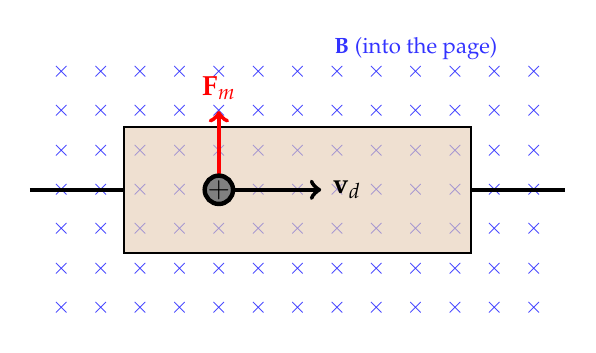
\begin{tikzpicture}
      \node at (4.5,3.8) {\textcolor{blue!80}{
          \footnotesize$\mb{B}$ (into the page)}
      };
      \foreach \x in {0,.5,...,6}{
        \foreach \y in {.5,1,...,3.5}{
          \node at (\x,\y) {\footnotesize\textcolor{blue!80}{$\times$}};
        }
      }
      \fill[brown!40,opacity=.6](.8,1.2) rectangle(5.2,2.8);
      \draw[thick](.8,1.2) rectangle(5.2,2.8);
      \draw[ultra thick](-.4,2)--(.8,2);
      \draw[ultra thick](5.2,2)--(6.4,2);

      \draw[->,ultra thick](2.18,2)--(3.3,2) node[pos=1,right]{$\mb{v}_d$};
      \draw[->,ultra thick,red](2,2.18)--(2,3) node[pos=1,above]{$\mb{F}_m$};
      \draw[ultra thick,fill=gray](2,2) circle(.18) node{$+$};
    \end{tikzpicture}
  \end{center}
  This is most evident in a \emph{thin}, \emph{flat} conductor as illustrated. 
\end{frame}



\begin{frame}{Magnetic Force}
  \begin{center}
    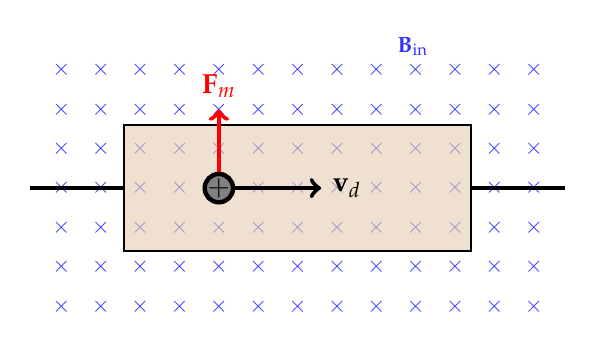
\begin{tikzpicture}
      \node at (4.5,3.8) {\textcolor{blue!80}{
          \footnotesize$\mb{B}_\mathrm{in}$
        }
      };
      \foreach \x in {0,.5,...,6}{
        \foreach \y in {.5,1,...,3.5}{
          \node at (\x,\y) {\footnotesize\textcolor{blue!80}{$\times$}};
        }
      }
      \fill[brown!40,opacity=.6](.8,1.2) rectangle(5.2,2.8);
      \draw[thick](.8,1.2) rectangle(5.2,2.8);
      \draw[ultra thick](-.4,2)--(.8,2);
      \draw[ultra thick](5.2,2)--(6.4,2);

      \draw[->,ultra thick](2.18,2)--(3.3,2) node[pos=1,right]{$\mb{v}_d$};
      \draw[->,ultra thick,red](2,2.18)--(2,3) node[pos=1,above]{$\mb{F}_m$};
      \draw[ultra thick,fill=gray](2,2) circle(.18) node{$+$};
    \end{tikzpicture}
  \end{center}
  \vspace{-.1in}As the charges enter the magnetic field, $\mb{F}_m$ is directed
  toward the top:
  
  \eq{-.2in}{
    \mb{F}_m
    =e\textcolor{red}{\mb{v}_d}\times\mb{B}
    =\frac{e\textcolor{red}{\mb{I}}\times\mb{B}}{\textcolor{red}{neA}}
  }

  leading to a surplus of positive charges on the top edge of
  the conductor, and negative charges on the bottom.
\end{frame}



\begin{frame}[t]{Hall Voltage}
  \begin{center}
    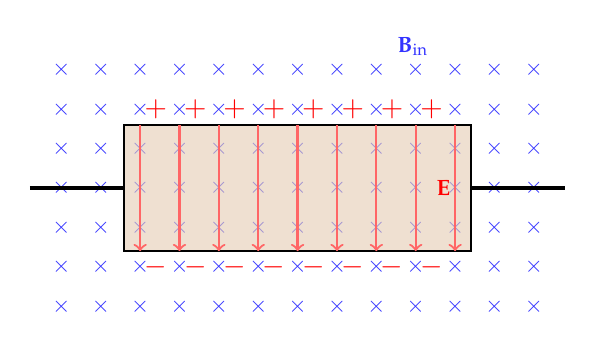
\begin{tikzpicture}
      \node at (4.5,3.8) {\textcolor{blue!80}{
          \footnotesize$\mb{B}_\mathrm{in}$
        }
      };
      \foreach \x in {0,.5,...,6}{
        \foreach \y in {.5,1,...,3.5}{
          \node at (\x,\y) {\footnotesize\textcolor{blue!80}{$\times$}};
        }
      }
      \fill[brown!40,opacity=.6](.8,1.2) rectangle(5.2,2.8);
      \draw[thick](.8,1.2) rectangle(5.2,2.8);
      \draw[ultra thick](-.4,2)--(.8,2);
      \draw[ultra thick](5.2,2)--(6.4,2);

      \foreach \x in {1.2,1.7,...,5}{ \node at (\x,1){\textcolor{red}{$-$}};}
      \foreach \x in {1.2,1.7,...,5}{ \node at (\x,3){\textcolor{red}{$+$}};}
      \foreach \x in {1,1.5,...,5}{
        \draw[thick,->,red!60] (\x,2.8)--(\x,1.2);
      }
      \node at (4.85,2) {\textcolor{red}{\footnotesize$\mb{E}$}};
    \end{tikzpicture}
  \end{center}
  The charge imbalance on the conductor creates an electric field $\mb{E}$,
  pointing toward the bottom, and therefore a voltage across two sides of the
  conductor (width $W$), called the \textbf{Hall voltage}:

  \eq{-.25in}{
    V_H=EW
  }
\end{frame}



\begin{frame}{Balancing Electrostatic \& Magnetic Forces}
  \begin{center}
    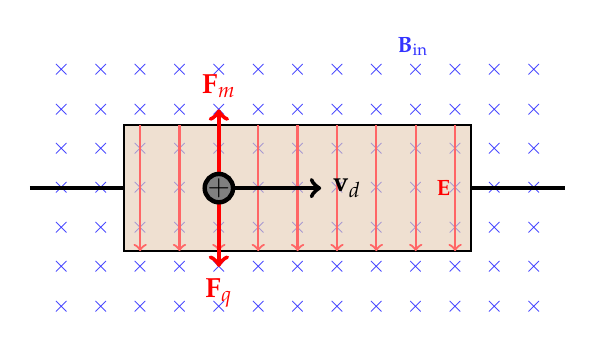
\begin{tikzpicture}
      \node at (4.5,3.8) {\textcolor{blue!80}{
          \footnotesize$\mb{B}_\mathrm{in}$
        }
      };
      \foreach \x in {0,.5,...,6}{
        \foreach \y in {.5,1,...,3.5}{
          \node at (\x,\y) {\footnotesize\textcolor{blue!80}{$\times$}};
        }
      }
      \fill[brown!40,opacity=.6](.8,1.2) rectangle(5.2,2.8);
      \draw[thick](.8,1.2) rectangle(5.2,2.8);
      \draw[ultra thick](-.4,2)--(.8,2);
      \draw[ultra thick](5.2,2)--(6.4,2);

      \foreach \x in {1,1.5,...,5}{
        \draw[thick,->,red!60] (\x,2.8)--(\x,1.2);
      }
      \node at (4.85,2) {\textcolor{red}{\footnotesize$\mb{E}$}};
      
      \draw[->,ultra thick](2.18,2)--(3.3,2) node[pos=1,right]{$\mb{v}_d$};
      \draw[->,ultra thick,red](2,2.18)--(2,3) node[pos=1,above]{$\mb{F}_m$};
      \draw[->,ultra thick,red](2,1.82)--(2,1) node[pos=1,below]{$\mb{F}_q$};
      \draw[ultra thick,fill=gray](2,2) circle(.18) node{$+$};
    \end{tikzpicture}
  \end{center}
  Subsequently, charge carriers entering the magnetic field will experience
  both a magnetic force and an electrostatic force. At equilibrium, the two
  forces are balanced:

  \eq{-.3in}{
    \mb{F}_m+\mb{F}_q=\mb{0}
  }
\end{frame}



\begin{frame}{Calculating Hall Voltage}
  The electrostatic force on the charge carrier can be expressed in terms of
  the Hall voltage $V_H$ across the two sides of the plate:

  \eq{-.15in}{
    F_q=eE=\frac{eV_H}{W}
  }
  
  Equating the magnitudes of electrostatic and magnetic forces, we can solve
  for the Hall voltage:

  \eq{-.2in}{
    F_m=F_q\quad\rightarrow\quad
    \frac{IB}{nA}=\frac{eV_H}{W}
  }
\end{frame}


\begin{frame}{Hall Voltage}
  Cancelling terms and noting that the thickness of the conductor is

  \eq{-.2in}{
    d=\frac{A}{W}
  }

  we find the expression for the Hall voltage $V_H$:

  \eq{-.1in}{
    \boxed{V_H=\frac{IB}{ned}}
  }
\end{frame}



\begin{frame}{Hall Probe}
  Large magnetic fields ($\sim$ \SI{1}{\tesla}) is often measured using a
  \textbf{Hall probe}. A thin film Hall probe is placed in the magnetic field
  and the transverse voltage (usually measured in on the order of
  \SI{e-6}{\volt}) is measured.

  \begin{center}
    \pic{.3}{hallp.png}
  \end{center}
  The polarity of the Hall voltage for a copper probe shows that electrons
  (negative charge) are the charge carriers.
\end{frame}
\end{document}
